%
% LaTeX Report Assignment 4
% Applied Programming Lab EE2703
% Ayush Jamdar EE20B018 
%


\documentclass[11pt, a4paper]{article}
\usepackage{graphicx}
\usepackage{amsmath}
\usepackage{listings}
\usepackage[]{courier}
%\usepackage{hyperref}


\title{Assignment 8: The Digital Fourier Transform} % Title

\author{Ayush Jamdar EE20B018} % Author name

\date{\today} % Date for the report
\begin{document}		
		
\maketitle % Insert the title, author and date
\section{Aim}
The goal of this assignment is to learn and apply the Digital Fourier Transform (DFT) using Python methods. The \texttt{numpy} library has the \texttt{fft} module that makes the analysis easier. 
  
\section{Introduction: DFT of $y=\sin(5x)$}
The sine function has two spectral lines at +1 and -1 in the frequency domain. 
$$\sin(x) = \frac{e^{jx}-e^{-jx}}{2j}$$
I am using $sin(5x)$ so lines at +-5. Start by computing the DFT of the sine function over a given range of $x$ in sampled time domain to sampled frequency domain in DFT. The line \texttt{Y = np.fft.fft(y) / 128} does this. Then I plot it to obtain Figure 1.
The code:
\begin{verbatim}
x = np.linspace(0, 2 * np.pi, 128)
y = np.sin(5 * x)
Y = np.fft.fft(y) / 128
plt.figure()
plt.subplot(2, 1, 1)
plt.plot(abs(Y), lw=2)
plt.title("Spectrum of signal y = sin(5x)")
plt.ylabel(r"$|Y|$", size=16)
plt.grid(True)
plt.subplot(2, 1, 2)
plt.plot(np.unwrap(np.angle(Y)), lw=2)
# unwrap adds multiples of ±2pi when the phase difference
# between consecutive elements of P are greater than or 
   equal to the jump threshold pi radians
plt.grid(True)
plt.ylabel(r"$\angle Y$", size=16)
plt.xlabel("$k$", size=16)
plt.savefig("a8\_1.png")
plt.show()


\end{verbatim} 
 
  \begin{figure}[!tbh]
   	\centering
  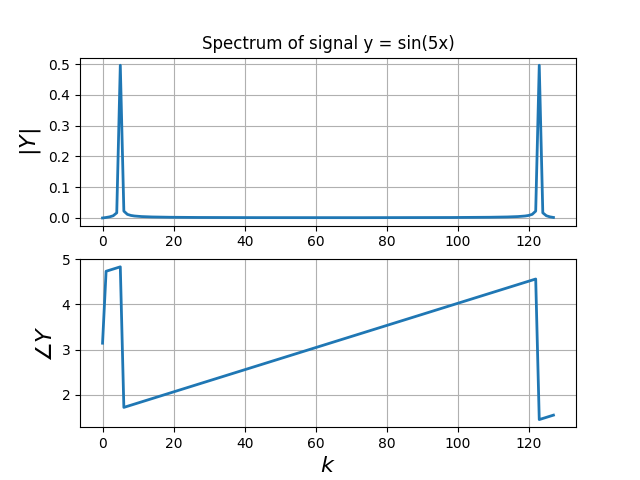
\includegraphics[scale=0.5]{a8_1.png} 
    \caption{Spectrum of $y=sin(x)$} 	
   \end{figure} 

This analysis is contrary to our understanding of the DFT as the spectral lines are not where one would expect. So I shift the part of the function from $\pi$ to $2\pi$ to the negative side as it represents negative frequencies (or say, $-\pi$ to $\pi$ is the same as $0$ to $2\pi$). This is done by \texttt{fftshift}. I have dropped the last element of the \texttt{x} array. This is because 0 and $2\pi$ are the same for sine. This is another update to this DFT. See Figure 2.
The code follows:
\begin{verbatim}
x = np.linspace(0, 2 * np.pi, 129)
x = x[:-1]  # remove the last element
y = np.sin(5 * x)
Y = np.fft.fftshift(np.fft.fft(y)) / 128
dft_plotter(Y, np.linspace(-64, 63, 128),
 func="sin(5x)", filename="a8_2.png")
\end{verbatim}
  
  The \texttt{DFT\_plotter} function just plots the magnitude and phase of the DFT. Note that it only uses the points with magnitude > 1e-3 in the phase plot. The \texttt{freq\_array} is the list of values of $k$ plotted on the x-axis.    
  The function:
  \begin{verbatim}
  def dft_plotter(dft_Y, freq_array, func, filename, xlim=15):
    plt.figure()
    plt.subplot(2, 1, 1)
    plt.plot(freq_array, abs(dft_Y), lw=2)
    plt.xlim([-xlim, xlim])
    plt.title("Spectrum of signal y = {}".format(func))
    plt.ylabel(r"$|Y|$", size=16)
    plt.grid(True)
    plt.subplot(2, 1, 2)
    ii = np.where(
        abs(dft_Y) > 1e-3
    )  # find the indices of the appreciably large elements
    plt.plot(freq_array[ii], np.angle(dft_Y[ii]), "go", lw=2)
    plt.xlim([-xlim, xlim])
    plt.grid(True)
    plt.ylabel(r"$\angle Y$", size=16)
    plt.xlabel(r"$k$", size=16)
    plt.savefig(filename)
    plt.show()
  \end{verbatim}
  \begin{figure}[!tbh]
   	\centering
  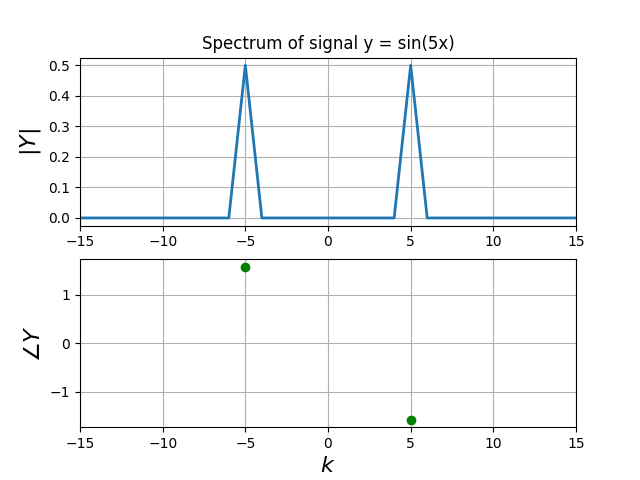
\includegraphics[scale=0.5]{a8_2.png} 
    \caption{Updated Spectrum of $y=sin(x)$} 	
   \end{figure} 
   
\subsection{Amplitude Modulation}
We will now find the spectrum of $$f(t)=(1+0.1\cos(t))\cos(10t)$$ 
If I proceed the same way as in the last question,
\begin{verbatim}
t = np.linspace(0, 2 * np.pi, 129)
t = t[:-1]  # remove the last element
y = (1 + 0.1 * np.cos(t)) * np.cos(10 * t)
Y = np.fft.fftshift(np.fft.fft(y)) / 128
w = np.linspace(-64, 63, 128)
dft_plotter(Y, w, func=r"$(1+0.1\cos(t))\cos(10t)$", 
   filename="a8_3.png")
\end{verbatim} 
\begin{figure}[!tbh]
   	\centering
  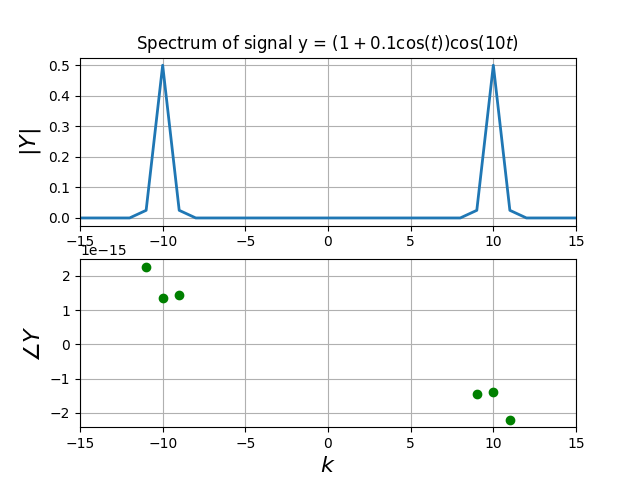
\includegraphics[scale=0.5]{a8_3.png} 
    \caption{Spectrum of AM Signal $f(t)=(1+0.1\cos(t))\cos(10t)$} 
   \end{figure} 
   
This gives Figure 3. But we lost two of the three peaks we expected at 9, 10, and 11 that should've appeared when two $\cos()$ of different frequencies are multiplied. The assignment told to use more samples, so instead I will use more samples (higher sampling frequency) in the frequency domain and same freq in the time domain. See Figure 4 the lines below:
\begin{verbatim}
t = np.linspace(-4 * np.pi, 4 * np.pi, 513)
t = t[:-1]  # remove the last element
y = (1 + 0.1 * np.cos(t)) * np.cos(10 * t)
Y = np.fft.fftshift(np.fft.fft(y)) / 512
w = np.linspace(-64, 64, 513)
w = w[:-1]  # remove the last element
dft_plotter(Y, w, func=r"$(1+0.1\cos(t))\cos(10t)$",
   filename="a8_4.png")
\end{verbatim}

\begin{figure}[!tbh]
   	\centering
  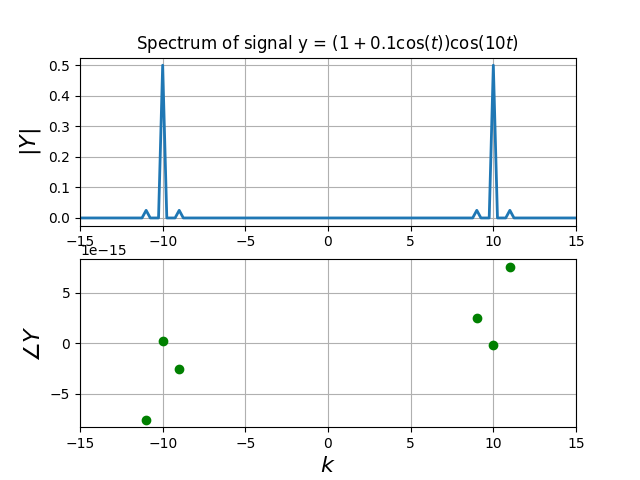
\includegraphics[scale=0.5]{a8_4.png} 
    \caption{Spectrum Of AM Signal at more samples} 	
   \end{figure} 


\subsection{Spectrum of $\sin^3t$ and $\cos^3t$}
Note that 
\begin{equation*}
    \sin^3(t) = \frac{3}{4}\sin(t) - \frac{1}{4}\sin(3t)
\end{equation*}
\begin{equation*}
    \cos^3(t) = \frac{3}{4}\cos(t) + \frac{1}{4}\cos(3t)
\end{equation*}
Thus one may expect four peaks in each of their plots. A similiar procedure as before, at higher sampling frequency in freq domain, is implemented in the below code:
\begin{verbatim}
# PART 3: Spectrum of sin^3t and cos^3t
t = np.linspace(-4 * np.pi, 4 * np.pi, 513)
t = t[:-1]  # remove the last element
y = np.sin(t) ** 3
Y = np.fft.fftshift(np.fft.fft(y)) / 512
w = np.linspace(-64, 64, 513)
w = w[:-1]  # remove the last element
dft_plotter(Y, w, func=r"$\sin^3t$", filename="a8_5.png")

t = np.linspace(-4 * np.pi, 4 * np.pi, 513)
t = t[:-1]  # remove the last element
y = np.cos(t) ** 3
Y = np.fft.fftshift(np.fft.fft(y)) / 512
w = np.linspace(-64, 64, 513)
w = w[:-1]  # remove the last element
dft_plotter(Y, w, func=r"$\cos^3t$", filename="a8_6.png")
\end{verbatim}

\begin{figure}[!tbh]
   	\centering
  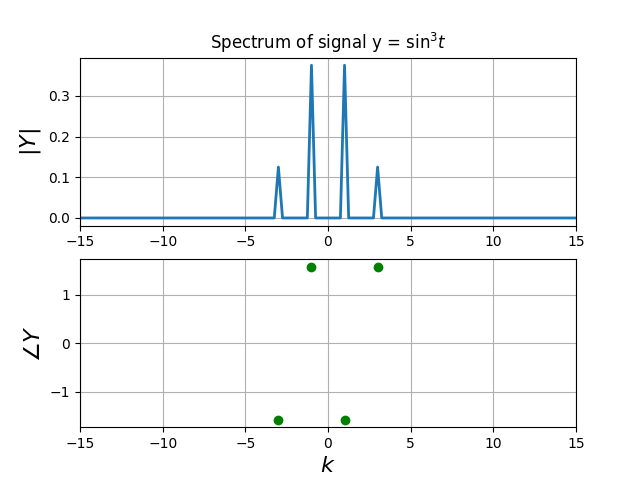
\includegraphics[scale=0.5]{a8_5.png} 
    \caption{Spectrum of $y=sin^3(t)$} 	
   \end{figure} 
   
   \begin{figure}[!tbh]
   	\centering
  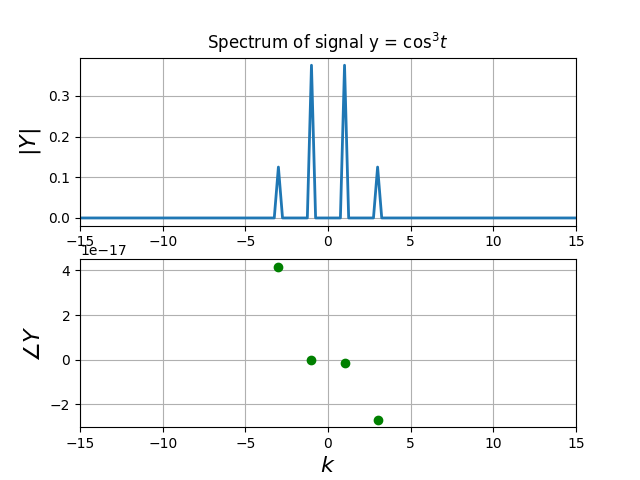
\includegraphics[scale=0.5]{a8_6.png} 
    \caption{Spectrum of $y=cos^3(t)$} 	
   \end{figure} 
   
\subsection{Spectrum of $\cos(20t+5\cos(t))$}
We find the spectrum of the following function:
\[f(t) = \cos(20t + 5\cos(t))\]
\begin{verbatim}
t = np.linspace(-4 * np.pi, 4 * np.pi, 513)
t = t[:-1]  # remove the last element
y = np.cos(20 * t + 5 * np.cos(t))
Y = np.fft.fftshift(np.fft.fft(y)) / 512
w = np.linspace(-64, 64, 513)
w = w[:-1]  # remove the last element
dft_plotter(Y, w, xlim=40, func=r"$\cos(20t+5\cos(t))$",
 filename="a8_7.png")
\end{verbatim}
The signal energy is distributed over a range of frequencies. This is Frequency Modulation. The carrier frequency is 20 here so the spectrum is centered at it. 

\begin{figure}[!tbh]
   	\centering
  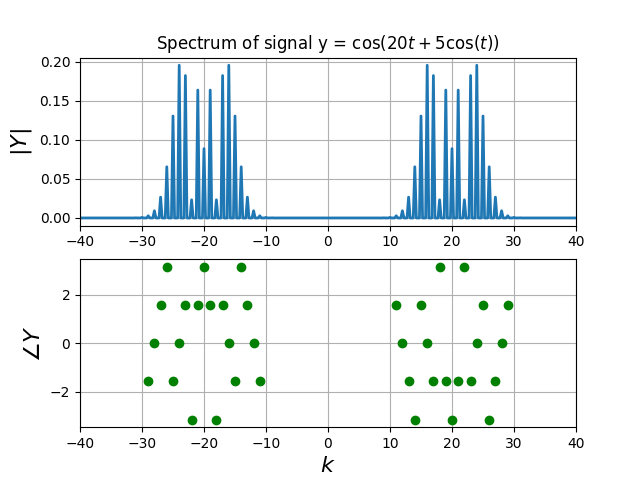
\includegraphics[scale=0.5]{a8_7.png} 
    \caption{Spectrum of $f(t)=\cos(20t+5\cos(t))$} 	
   \end{figure} 
   
\subsection{DFT of a Gaussian}
$$f(t)=e^{-t^2/2}$$
$$F(\omega)=\sqrt{2\pi}e^{-\omega^2/2} $$
The phase should be zero for all frequency samples and the magnitude plot should look like a Gaussian distribution. The goal is to obtain a set of \texttt{tlim}, \texttt{wlim}, and number of samples \texttt{N} such that the error - difference of the values of the DFT obtained after \texttt{fft.fft()} and the ones calculated directly from the formula - should be lower than $10^{-6}$.  I have tried different sets of values. First with $tlim = 4\pi$, $wlim=64$ and 512 samples. Then with $8\pi$, 32 and 512. 
\begin{verbatim}
# Take - 1: tlim=4pi, wlim=64, N=512
t = np.linspace(-4 * np.pi, 4 * np.pi, 513)
t = t[:-1]  # remove the last element
y = np.exp(-(t**2) / 2)
Y = abs(np.fft.fftshift((np.fft.fft(y)))) / 512
Y = Y * np.sqrt(2 * np.pi) / np.max(Y)
w = np.linspace(-64, 64, 513)
w = w[:-1]  # remove the last element
Y_actual = np.sqrt(2 * np.pi) * np.exp(-(w**2) / 2)
print("Max Error = {}".format((abs(Y - Y_actual).max())))
dft_plotter(Y, w, xlim=15, func=r"$\exp(-t^2/2)$",
 filename="a8_8.png")

# Take - 2: tlim=8pi, wlim=32, N=512
t = np.linspace(-8 * np.pi, 8 * np.pi, 513)
t = t[:-1]  # remove the last element
y = np.exp(-(t**2) / 2)
# Normalise the spectrum
Y = np.fft.fftshift(abs(np.fft.fft(y))) / 512
Y = Y * np.sqrt(2 * np.pi) / np.max(Y)
w = np.linspace(-32, 32, 513)
w = w[:-1]  # remove the last element
Y_actual = np.sqrt(2 * np.pi) * np.exp(-(w**2) / 2)
print("Max Error = {}".format(np.max(abs(Y - Y_actual))))
dft_plotter(Y, w, xlim=15, func=r"$\exp(-t^2/2)$",
 filename="a8_9.png")
\end{verbatim}

\begin{figure}[!tbh]
   	\centering
  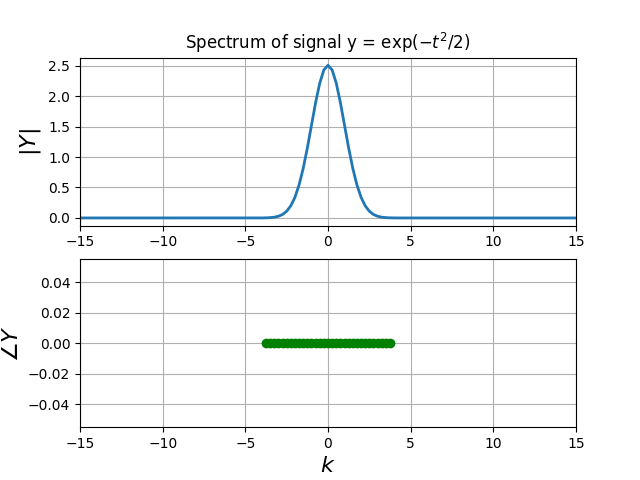
\includegraphics[scale=0.5]{a8_8.png} 
    \caption{tlim=4$\pi$, wlim=64, N=512} 	
   \end{figure} 

\begin{figure}[!tbh]
   	\centering
  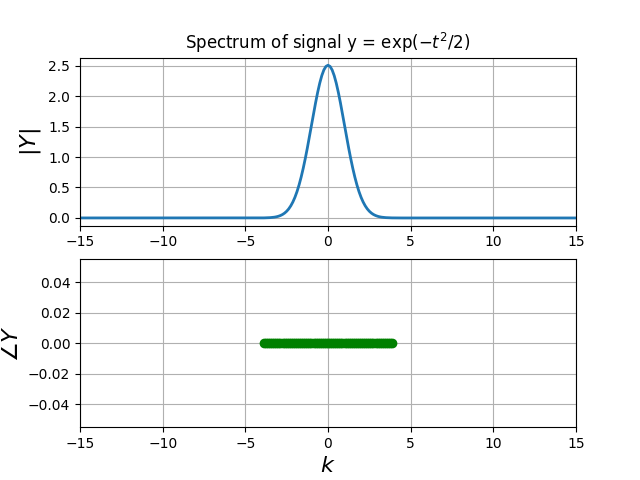
\includegraphics[scale=0.5]{a8_9.png} 
    \caption{tlim=8$\pi$, wlim=32, N=512} 	
   \end{figure} 
   
The error here is of the order $10^-{15}$ which is already within the required limits. What if I use 8$\pi$, 64 and 512 (Take-3). That is, just increase tlim with respect to Take-1. It gives an error of around 1.18, substantially large than in Take-1. This means reducing sampling frequency in time domain increases the error. The plots for different trials are attached here. One can compare combinations of two plots to see the effect of one parameter. Now see Take-3 and Take-4 where wlim decreases. Error also decreases (See Python).  


\begin{figure}[!tbh]
   	\centering
  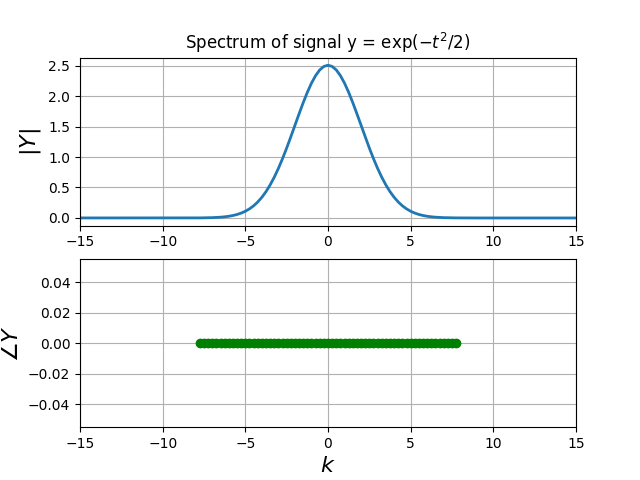
\includegraphics[scale=0.5]{a8_10.png} 
    \caption{tlim=8$\pi$, wlim=64, N=512} 	
   \end{figure} 
   
   
\begin{figure}[!tbh]
   	\centering
  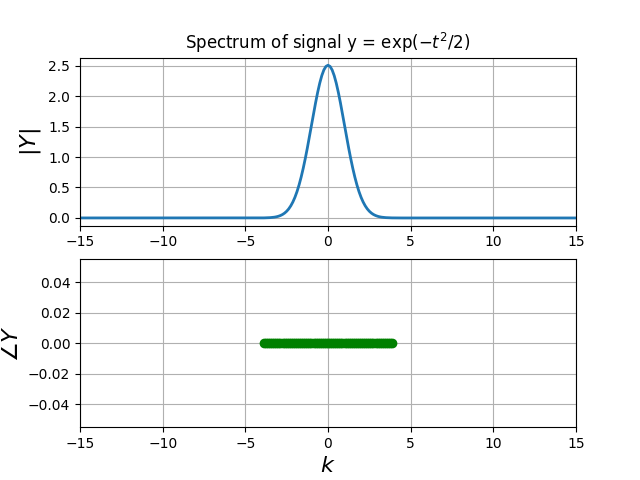
\includegraphics[scale=0.5]{a8_11.png} 
    \caption{tlim=8$\pi$, wlim=32, N=512} 	
   \end{figure} 
   
   
\begin{figure}[!tbh]
   	\centering
  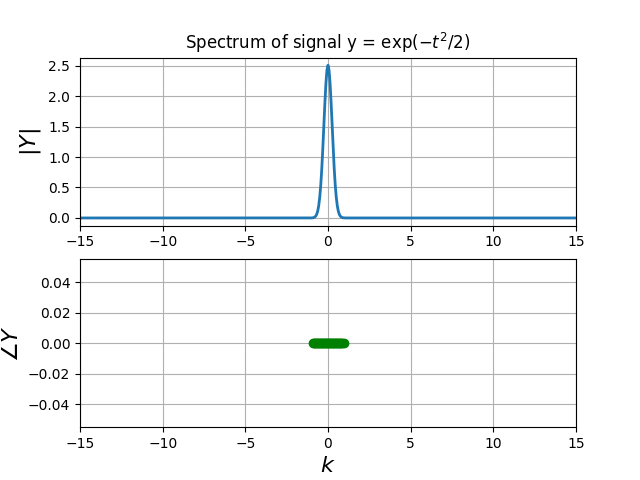
\includegraphics[scale=0.5]{a8_12.png} 
    \caption{tlim=4$\pi$, wlim=32, N=1024} 	
   \end{figure}   

\section{Conclusion}
The aim that we took at the beginning of this assignment is now seen to have been accomplished. We explored the \texttt{numpy.fft} module by using it to find the Fourier and Inverse Fourier Transforms of various signals. We learnt about the DFT and implementing it using \texttt{fft.fft()}. 




\end{document}